%************************************************
\chapter{User Guide}\label{ch:user_guide} % $\mathbb{ZNR}$
%************************************************

This chapter will describe how to access the five functionalities provided by the application via its \ac{GUI}:

\begin{itemize}
\item Requesting and displaying web-pages.
\item Managing the history of requested web-pages.
\item Managing user-defined favourites.
\item Managing a user-defined home-page.
\item Allow printing of the currently displayed web-page.
\end{itemize}

\section{Requesting a web-page}
\label{sec:request_web_page}

Upon starting the application the user will see the following window:

\begin{figure}[H]
\begin{center}
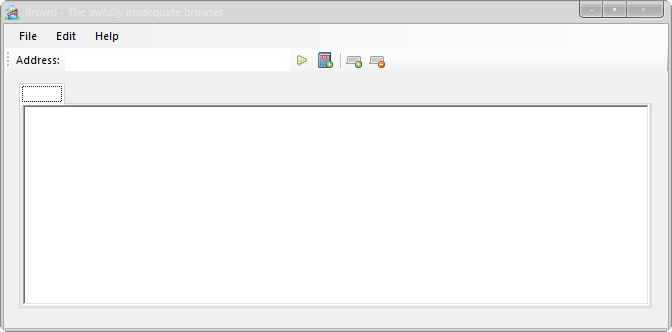
\includegraphics[width=\textwidth]{gfx/main_window.png}
\caption{The application's main window.}
\label{fig:main_window}
\end{center}
\end{figure}

To request a web-page the user must enter the desired address in the \texttt{Address} text-box and then press the \texttt{Go}-button (\raisebox{-1mm}{
\includegraphics{gfx/16-arrow-right.png}}).

The format of the entered address will be verified. It must match the following pattern\footnote{Parts in square-brackets may not be required for all web-pages.}:

\begin{lstlisting}[language=xml]
http://[www.]address.domain[/url-path]
\end{lstlisting}

Should the entered address not match the format of a valid web-address, the program will notify the user about the error by displaying a message-box:

\begin{figure}[H]
\begin{center}
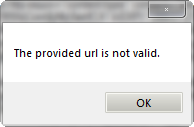
\includegraphics[scale=1]{gfx/error_message.png}
\caption{Error message due to invalid url.}
\label{fig:error_message}
\end{center}
\end{figure}

When the url is valid the browser will display the \ac{HTML}-code in the current tab:

\begin{figure}[H]
\begin{center}
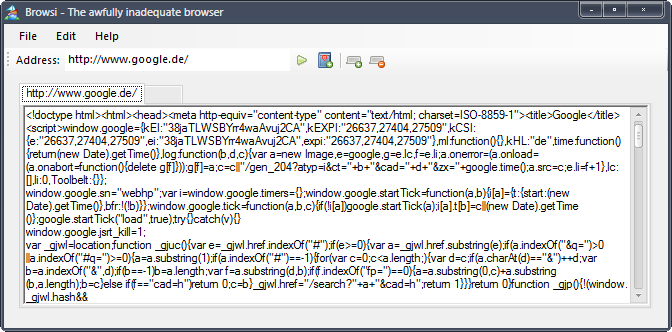
\includegraphics[width=\textwidth]{gfx/display_page.png}
\caption{Browser displaying the current web-page.}
\label{fig:display_page}
\end{center}
\end{figure}

To request multiple pages simultaneously it is possible to utilize tabs:

To create a new tab, the user simply presses the \texttt{AddTab}-button (\raisebox{-1mm}{
\includegraphics{gfx/tab_add.png}}). This will create new (and empty) tab-page.

Should the user want to close a tab it is necessary to select the tab that should be closed and press the \texttt{RemoveTab}-button (\raisebox{-1mm}{
\includegraphics{gfx/tab_delete.png}}).

\section{Managing the history}
\label{sec:managing_history}

Every web-page requested by the user will be saved in the \texttt{history}.

The history can be accessed by pressing the \texttt{History}-button (\raisebox{-1mm}{
\includegraphics{gfx/calendar.png}}) in the \texttt{MenuBar} under \texttt{Edit $\rightarrow$ History}.

This will display a panel in the main window of the application that shows the \texttt{History} in one and the \texttt{Favourites} in another tab:

\begin{figure}[H]
\begin{center}
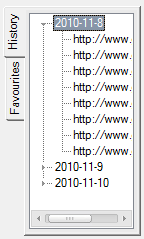
\includegraphics[scale=1]{gfx/history.png}
\caption{The history tab.}
\label{fig:history_tab}
\end{center}
\end{figure}

As can be seen the history is ordered in a tree-structure that groups together addresses that were visited on the same day.

To visit one of the pages the user just double-clicks one of the links in the tree and the application will open the requested page in the current tab.

As the history is prone to become quite huge it is possible to clear it. To perform this action the user selects the \texttt{ClearHistory}-option (\raisebox{-1mm}{
\includegraphics{gfx/calendar_delete.png}}) from the \texttt{MenuBar}. This operation can be found under \texttt{Edit $\rightarrow$ History $\rightarrow$ Clear}.

\section{Managing favourites}
\label{sec:managing_favourites}

The application allows a user to add, edit and delete favourites.

There are two ways to add a favourite: either the user clicks the \texttt{AddFavourite}-button (\raisebox{-1mm}{
\includegraphics[scale=2]{gfx/bookmark_add.png}}) in the \texttt{AddressBar} or in the \texttt{ContextMenu} of the Favourites-List.

To open the \texttt{Favourites-List} the user clicks the \texttt{Favourite}-button in the \texttt{MenuBar}: \texttt{Edit $\rightarrow$ Favourites}.

This will open the Favourites-List:

\begin{figure}[H]
\begin{center}
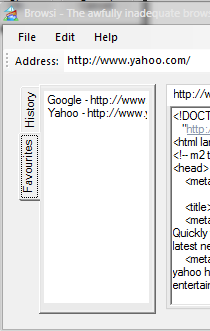
\includegraphics[scale=1]{gfx/favourites.png}
\caption{The favourites tab.}
\label{fig:favourites_tab}
\end{center}
\end{figure}

When the user right-clicks in this list a context-menu will open that will allow the user to either \texttt{Add}, \texttt{Edit} or \texttt{Delete} a favourite.

\begin{figure}[H]
\begin{center}
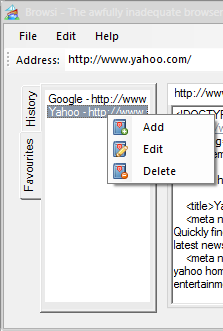
\includegraphics[scale=1]{gfx/context_menu.png}
\caption{The context menu.}
\label{fig:context_menu}
\end{center}
\end{figure}

When the user decides to add a favourite, a new window will pop-up that asks him to enter a name and a \ac{URL} for the favourite. The \ac{URL} will, by default, be set to the address of the currently activated tab.

\begin{figure}[H]
\begin{center}
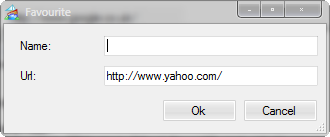
\includegraphics[scale=1]{gfx/add_favourite.png}
\caption{Add-favourite window.}
\label{fig:add_favourite}
\end{center}
\end{figure}

\section{Setting a home-page}
\label{sec:setting_home_page}

It is also possible to set a home-page that will be opened as soon as the application is started.

Therefore the user opens the \texttt{Settings}-Window by clicking on the \texttt{Settings}-button (\raisebox{-1mm}{
\includegraphics{gfx/wrench_orange.png}}) found under \texttt{File $\rightarrow$ Settings}.

This will open the \texttt{Settings}-Window that allows the user to enter a home-page:

\begin{figure}[H]
\begin{center}
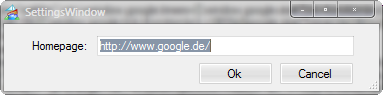
\includegraphics[scale=1]{gfx/settings_menu.png}
\caption{Settings window.}
\label{fig:settings_window}
\end{center}
\end{figure}

\section{Printing a web-page}
\label{sec:printing_web_page}

The last function the user can perform is to print a web-page.

Therefore the tab that should be printed needs to be selected and then the \texttt{Print}-button (\raisebox{-1mm}{
\includegraphics{gfx/printer.png}}) needs to be clicked (\texttt{File $\rightarrow$ Print}).

This will display a print-dialog that allows the user to tweak desired settings:

\begin{figure}[H]
\begin{center}
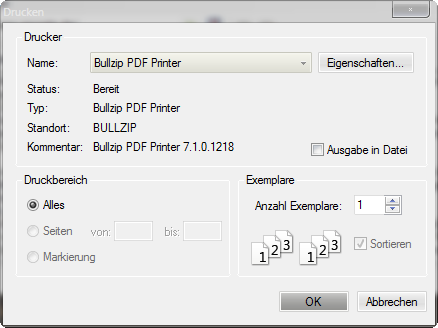
\includegraphics[scale=1]{gfx/print_dialog.png}
\caption{Common windows print-dialog.}
\label{fig:print_dialog}
\end{center}
\end{figure}

Clicking the \texttt{OK}-button will the print the \ac{HTML} of the current tab.

